\subsection{Masking}
\label{sec:masking}


To address Q1 (Hallucination-free listening) and Q2 (Wholistic listening), we apply \textit{Random Masking} and \textit{Guided Masking} to evaluate if models stay grounded in the actual audio signal. We achieve this by removing or isolating specific components of the audio input and observing the impact on the model's CoT and final predictions.

\noindent \textbf{Setup:} 
For \textit{Random Masking}, we mask [20\%, 40\%, 60\%, 80\%, and 100\%] of the audio in distributed chunks. For tasks focusing on global features, such as predicting an animal, gender, or emotion rather than specific speech content, randomized masking should not disproportionately affect performance unless the model relies on specific "attention sinks" or hidden encoded representations within a narrow segment of the audio. By distributing masks across the entire duration, we ensure the model cannot rely on a single localized "shortcut" and instead must attentively listen to the entire audio context. At 100\% masking (total silence), we evaluate Q1 to determine if the model produces hallucinatory reasoning when no signal is present. 

We further utilize \textit{Guided Masking} on the JASCO dataset \cite{wang2025they} to investigate how models attend to different modalities (speech vs. audio). Following the original evaluation pipeline \cite{wang2025they}, we use an LLM-as-a-judge (\texttt{Mistral-Small-3.1-24B-Instruct-2503}) with a three-tier scoring system to compare model predictions against reference answers. To determine modality dependency, the judge evaluates whether the model’s final reasoning is drawn from both modalities or a single source. By specifically masking either the speech segments (\textit{Speech Mask}) or the general background sounds (\textit{Audio Mask}), we force the model to shift its reasoning based on the remaining modality, testing whether it achieves true joint audio-speech understanding or relies on a single dominant source.


\newcommand{\figsize}{0.19}
\begin{figure*}[t]
    \centering
    % Row 0: Legend
    
\includegraphics[width=0.8\linewidth]{figures/audio_intervention/legend_datasets_only.pdf}
    
    \vspace{-.3cm}

    % Row 1 Header: Labels for Columns
    %\begin{minipage}{0.24\textwidth}\centering \small \textbf{Paraphrasing}\end{minipage}
    %\begin{minipage}{0.24\textwidth}\centering \small \textbf{Early Answering}\end{minipage}
    %\begin{minipage}{0.24\textwidth}\centering \small \textbf{Adding Mistake}\end{minipage}
    %\begin{minipage}{0.24\textwidth}\centering \small \textbf{Filler Token}\end{minipage}

    \vspace{-.5cm}

    % Row 1: AF3 Plots
    \rotatebox{90}{\makebox[0.18\textwidth]{\small \textbf{AF3}}} %\hfill
    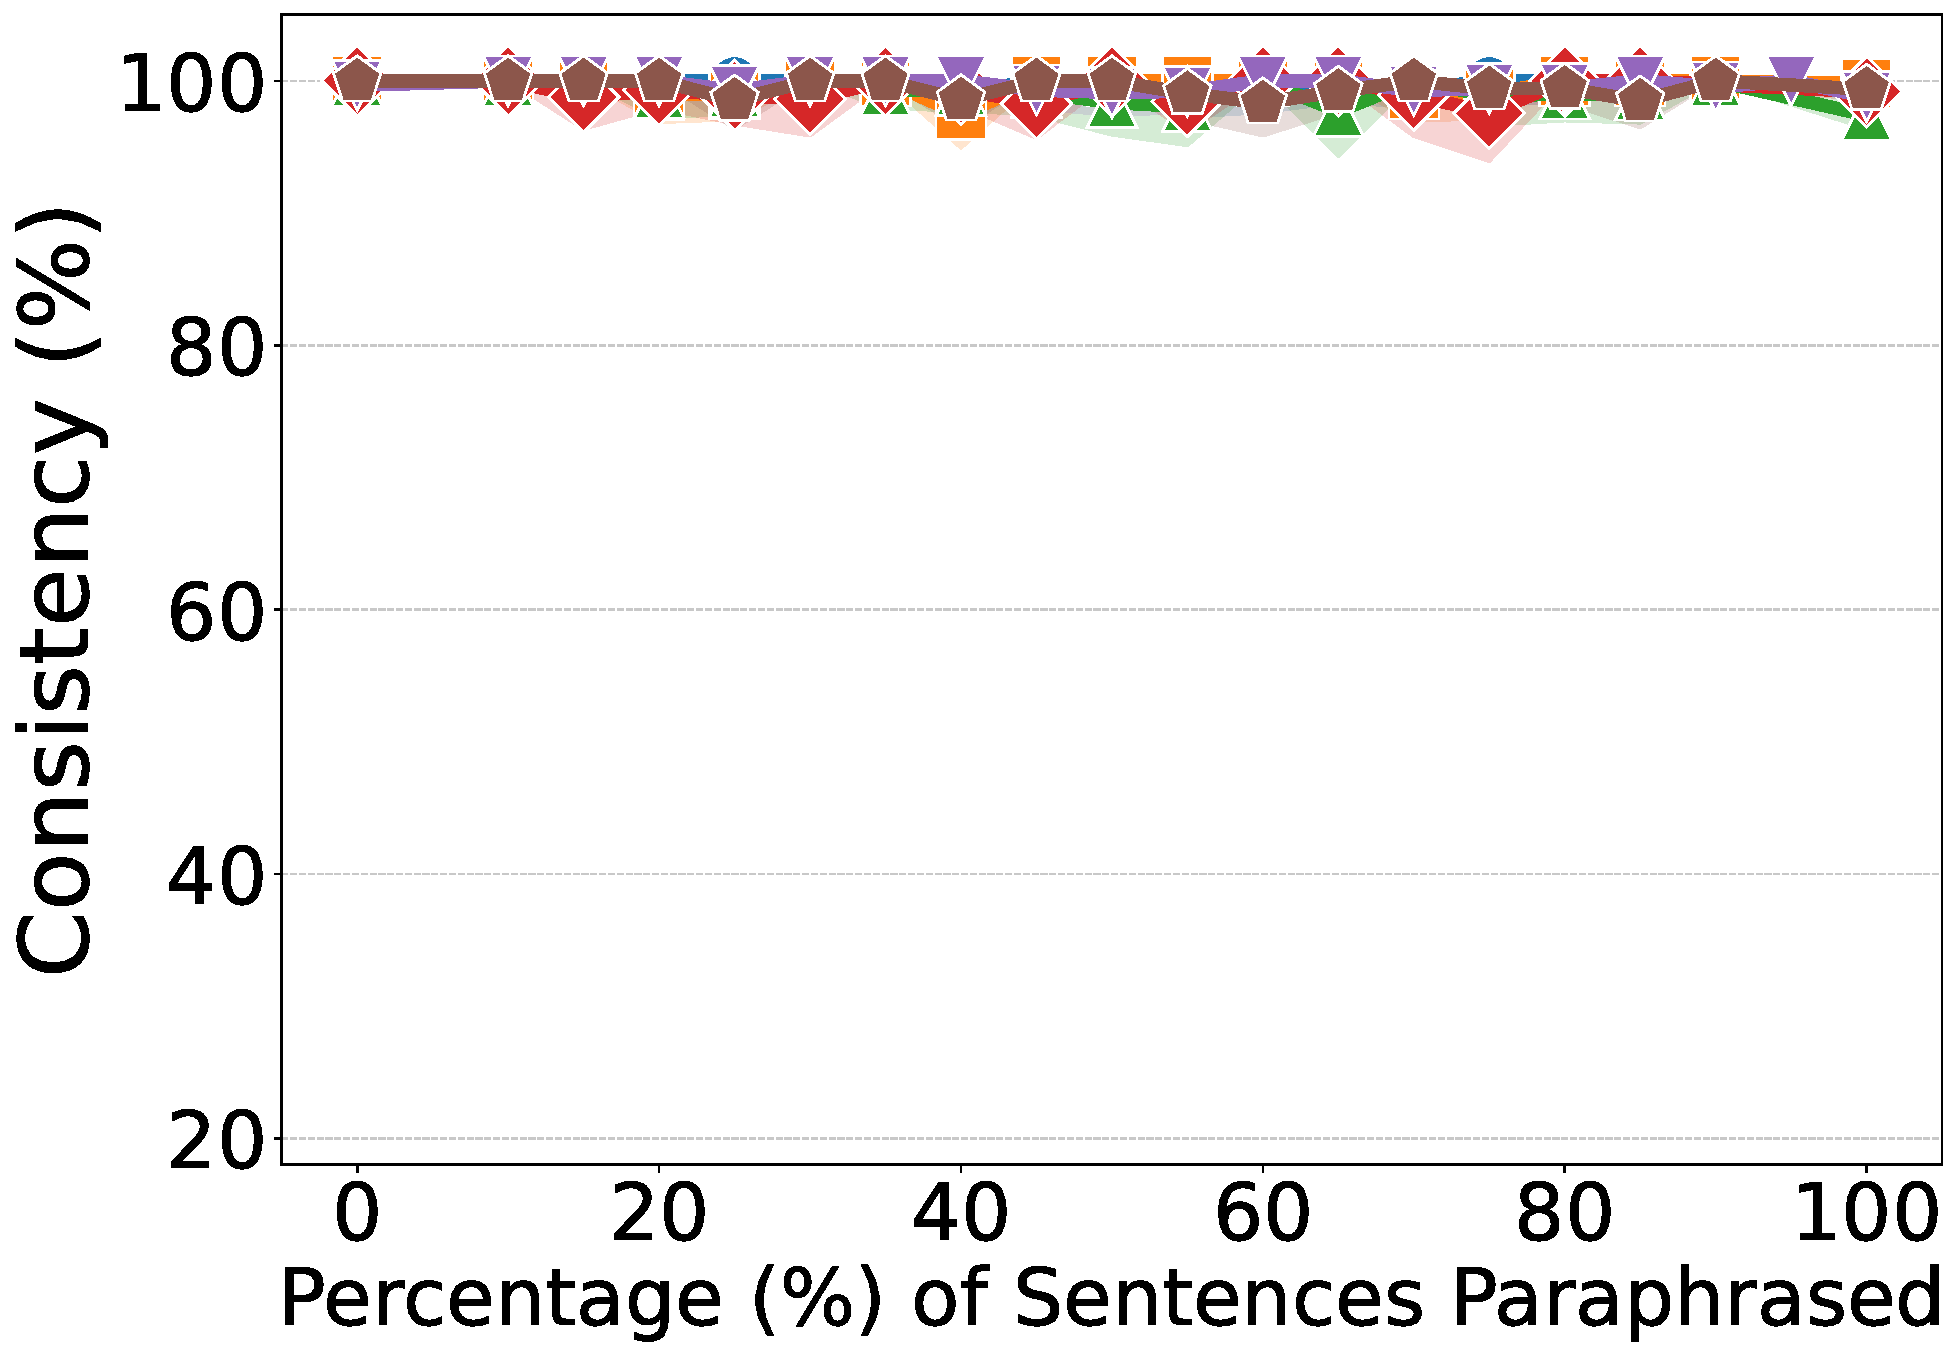
\includegraphics[width=\figsize\textwidth]{figures/cot_intervention/flamingo_hf/paraphrasing/cross_dataset_paraphrasing_0pct_words_flamingo_hf_restricted-mistral.pdf} %\hfill
    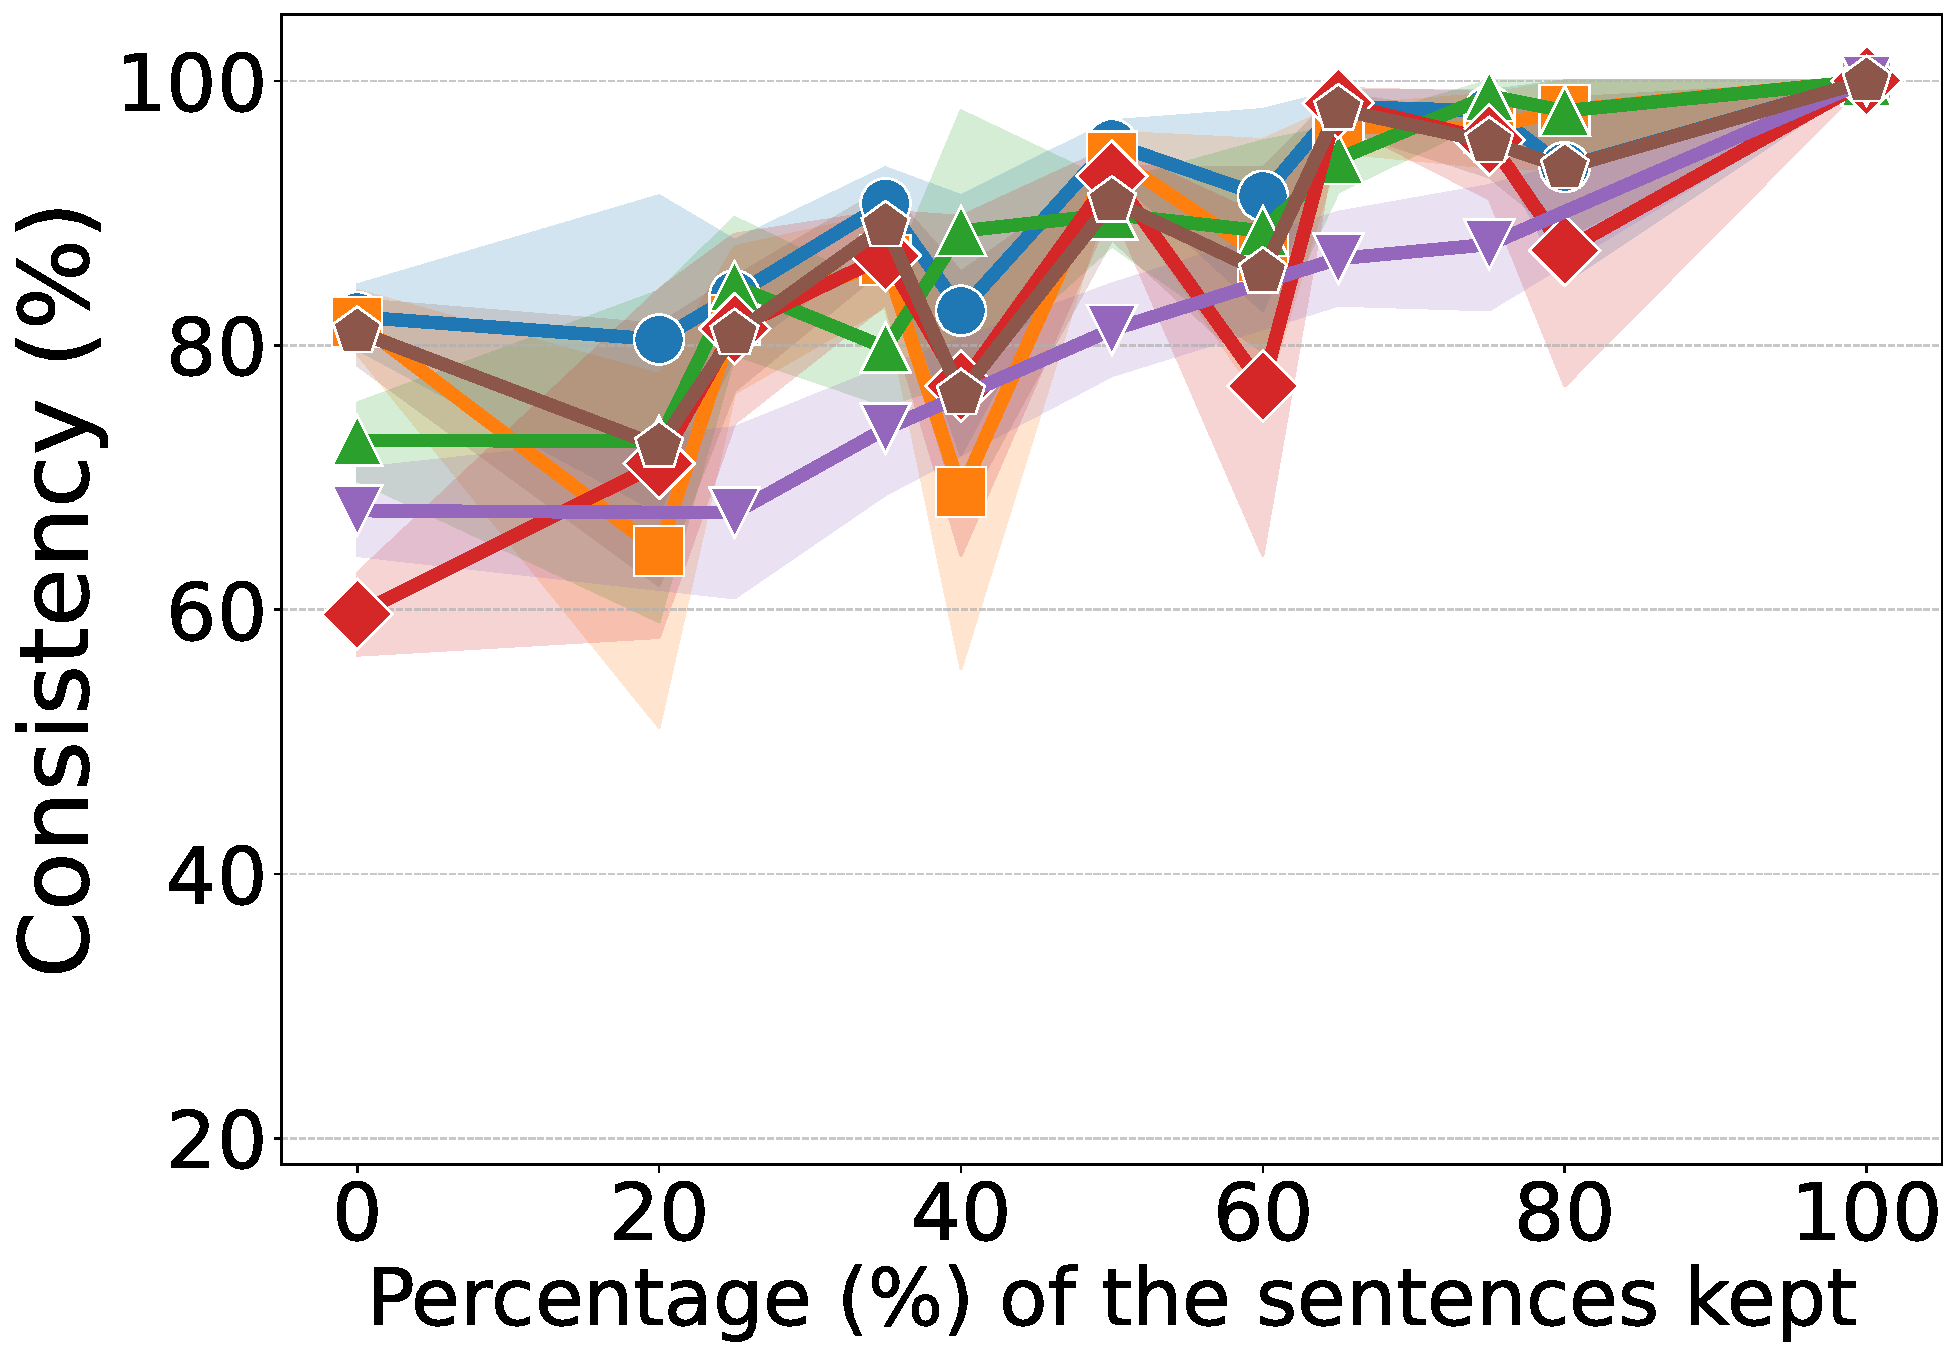
\includegraphics[width=\figsize\textwidth]{figures/cot_intervention/flamingo_hf/early_answering/cross_dataset_early_answering_100pct_flamingo_hf_restricted.pdf} %\hfill
    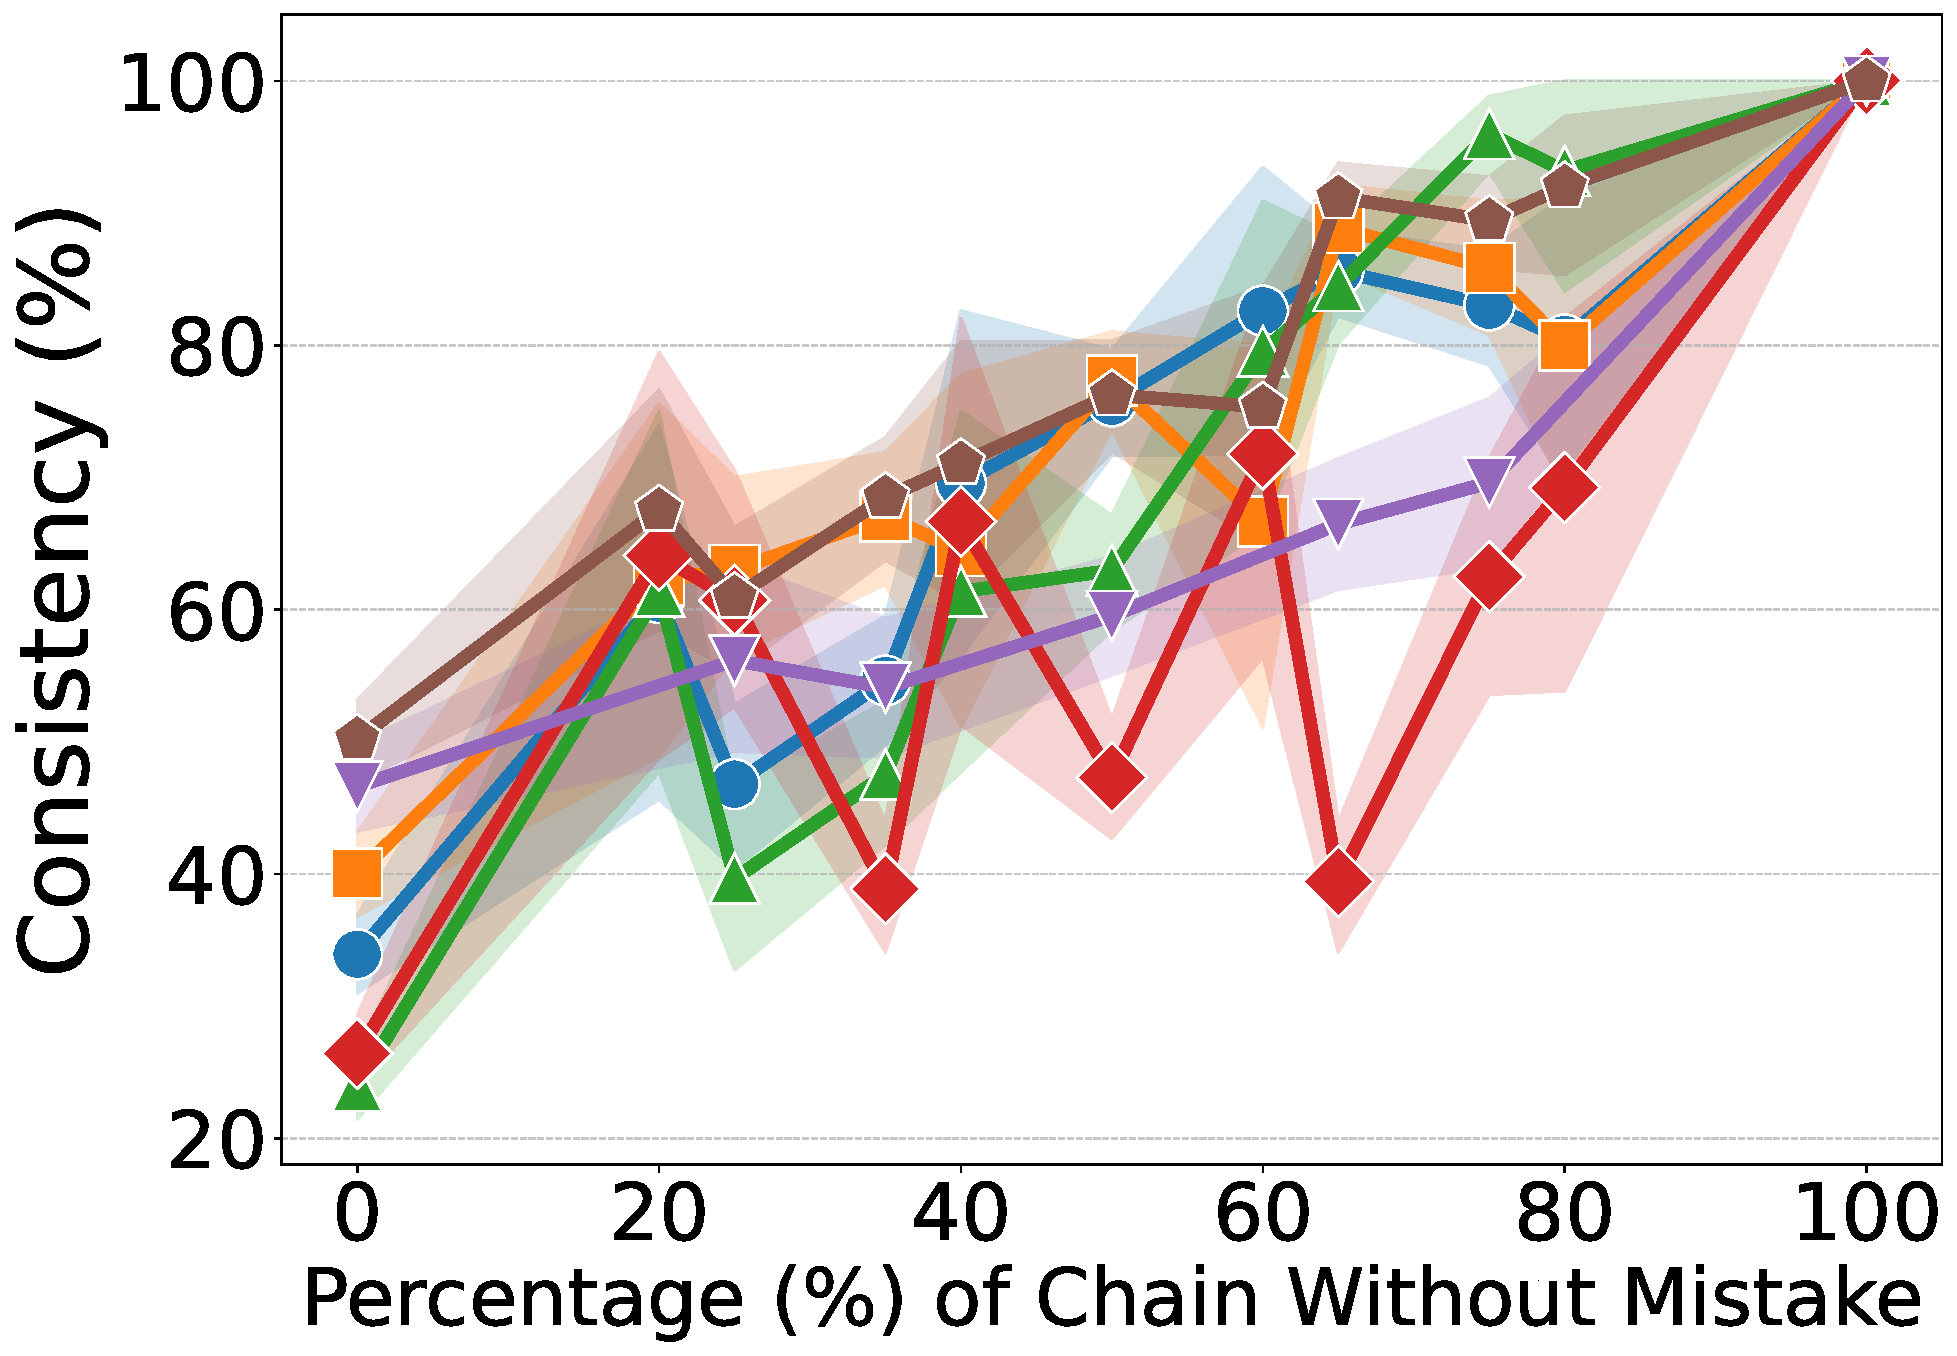
\includegraphics[width=\figsize\textwidth]{figures/cot_intervention/flamingo_hf/adding_mistakes/cross_dataset_adding_mistakes_vs_rpf_flamingo_hf_restricted-mistral.pdf} %\hfill
    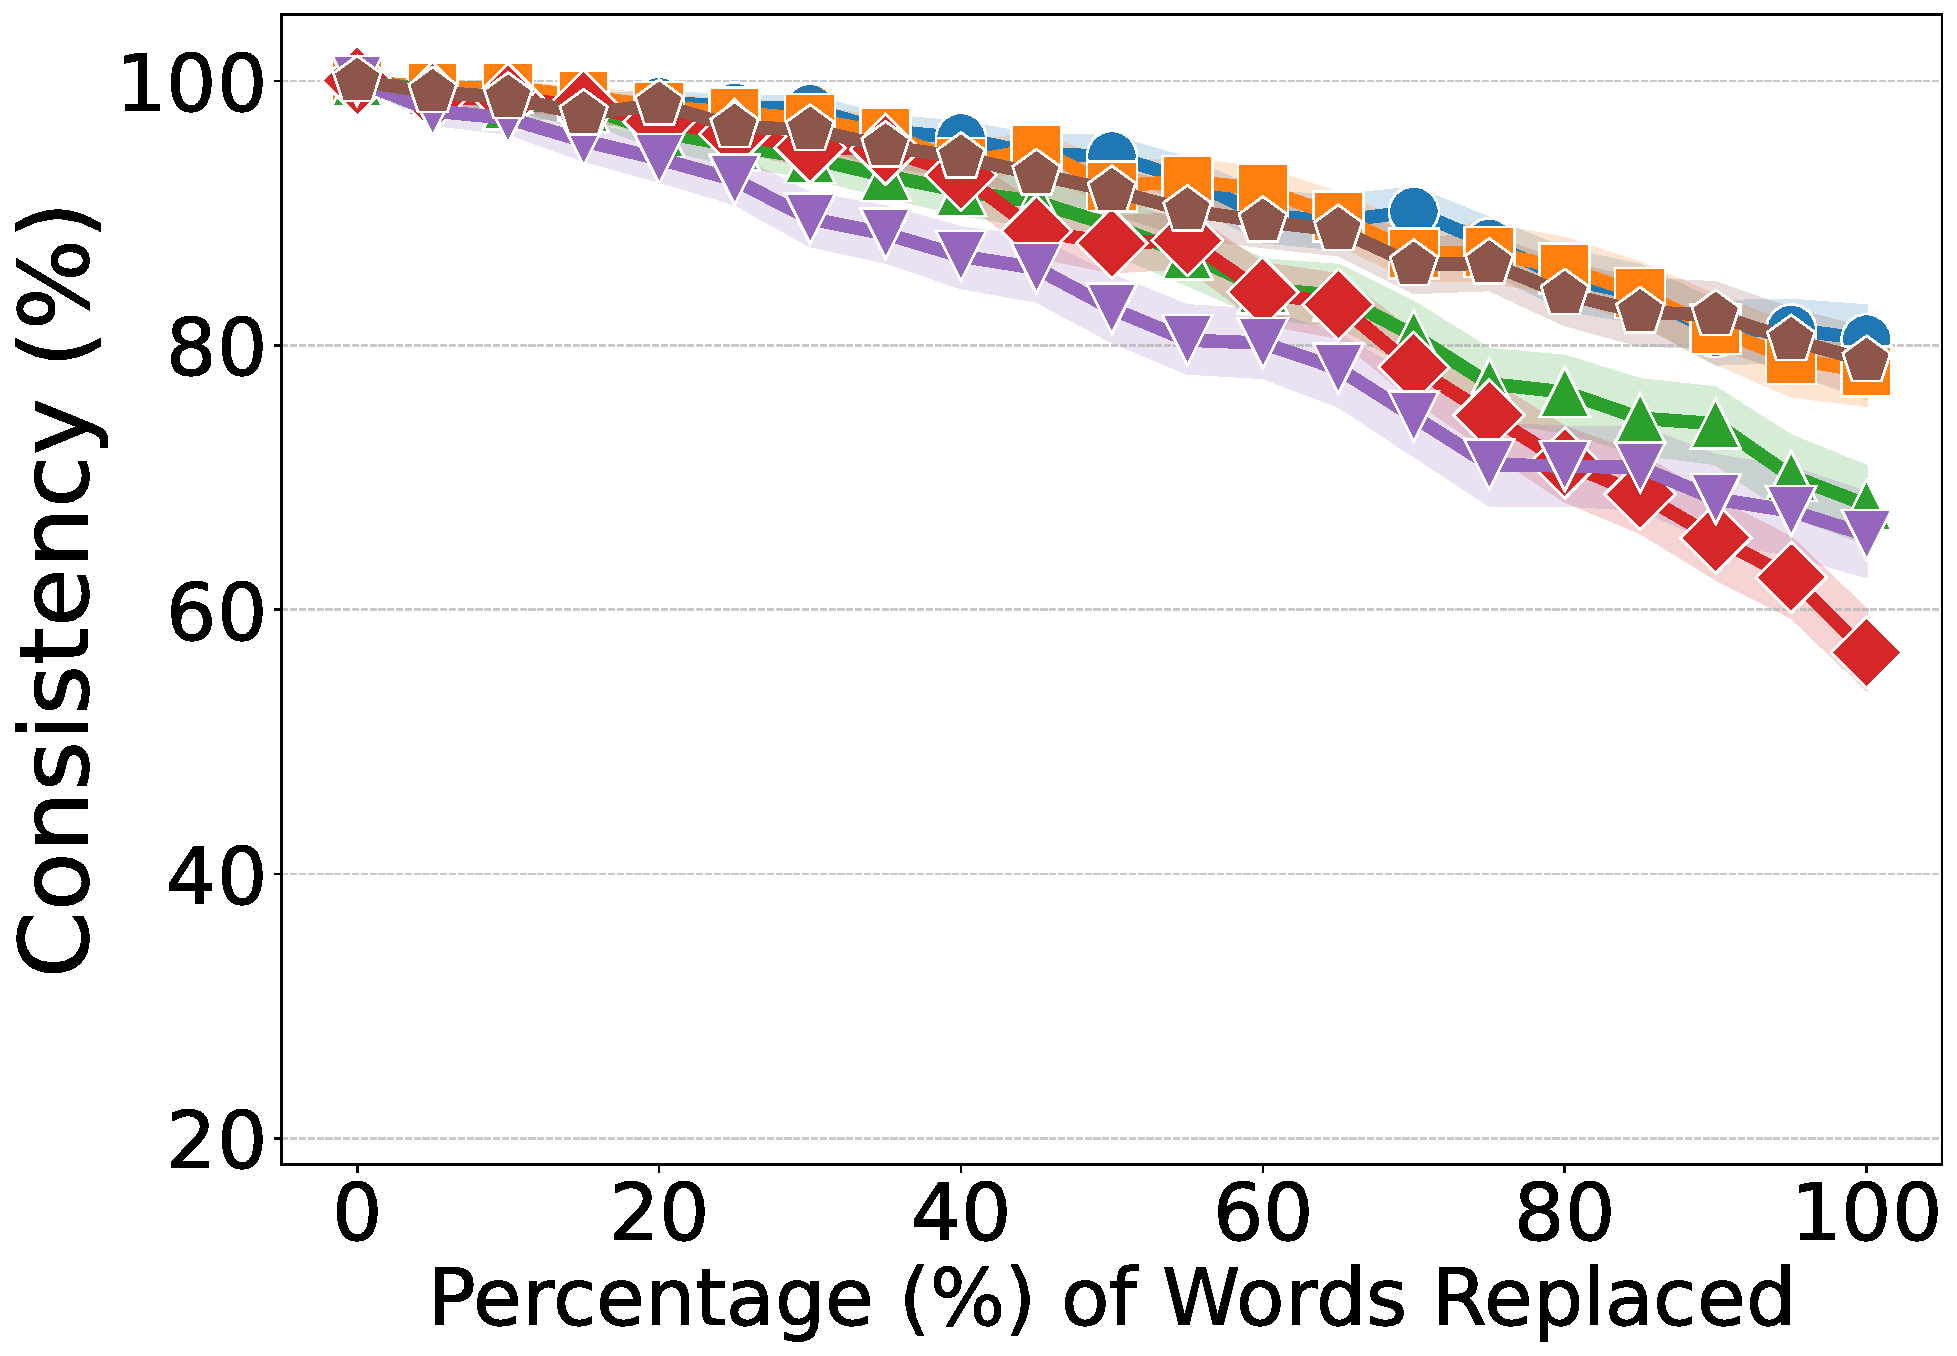
\includegraphics[width=\figsize\textwidth]{figures/cot_intervention/flamingo_hf/random_partial_filler_text/cross_dataset_random_partial_filler_text_0pct_flamingo_hf_lorem_restricted.pdf}

    \vspace{-0.6cm}

    % Row 2: Qwen2.5-Omni Plots
    \rotatebox{90}{\makebox[0.18\textwidth]{\small \textbf{Qwen2.5}}} %\hfill
    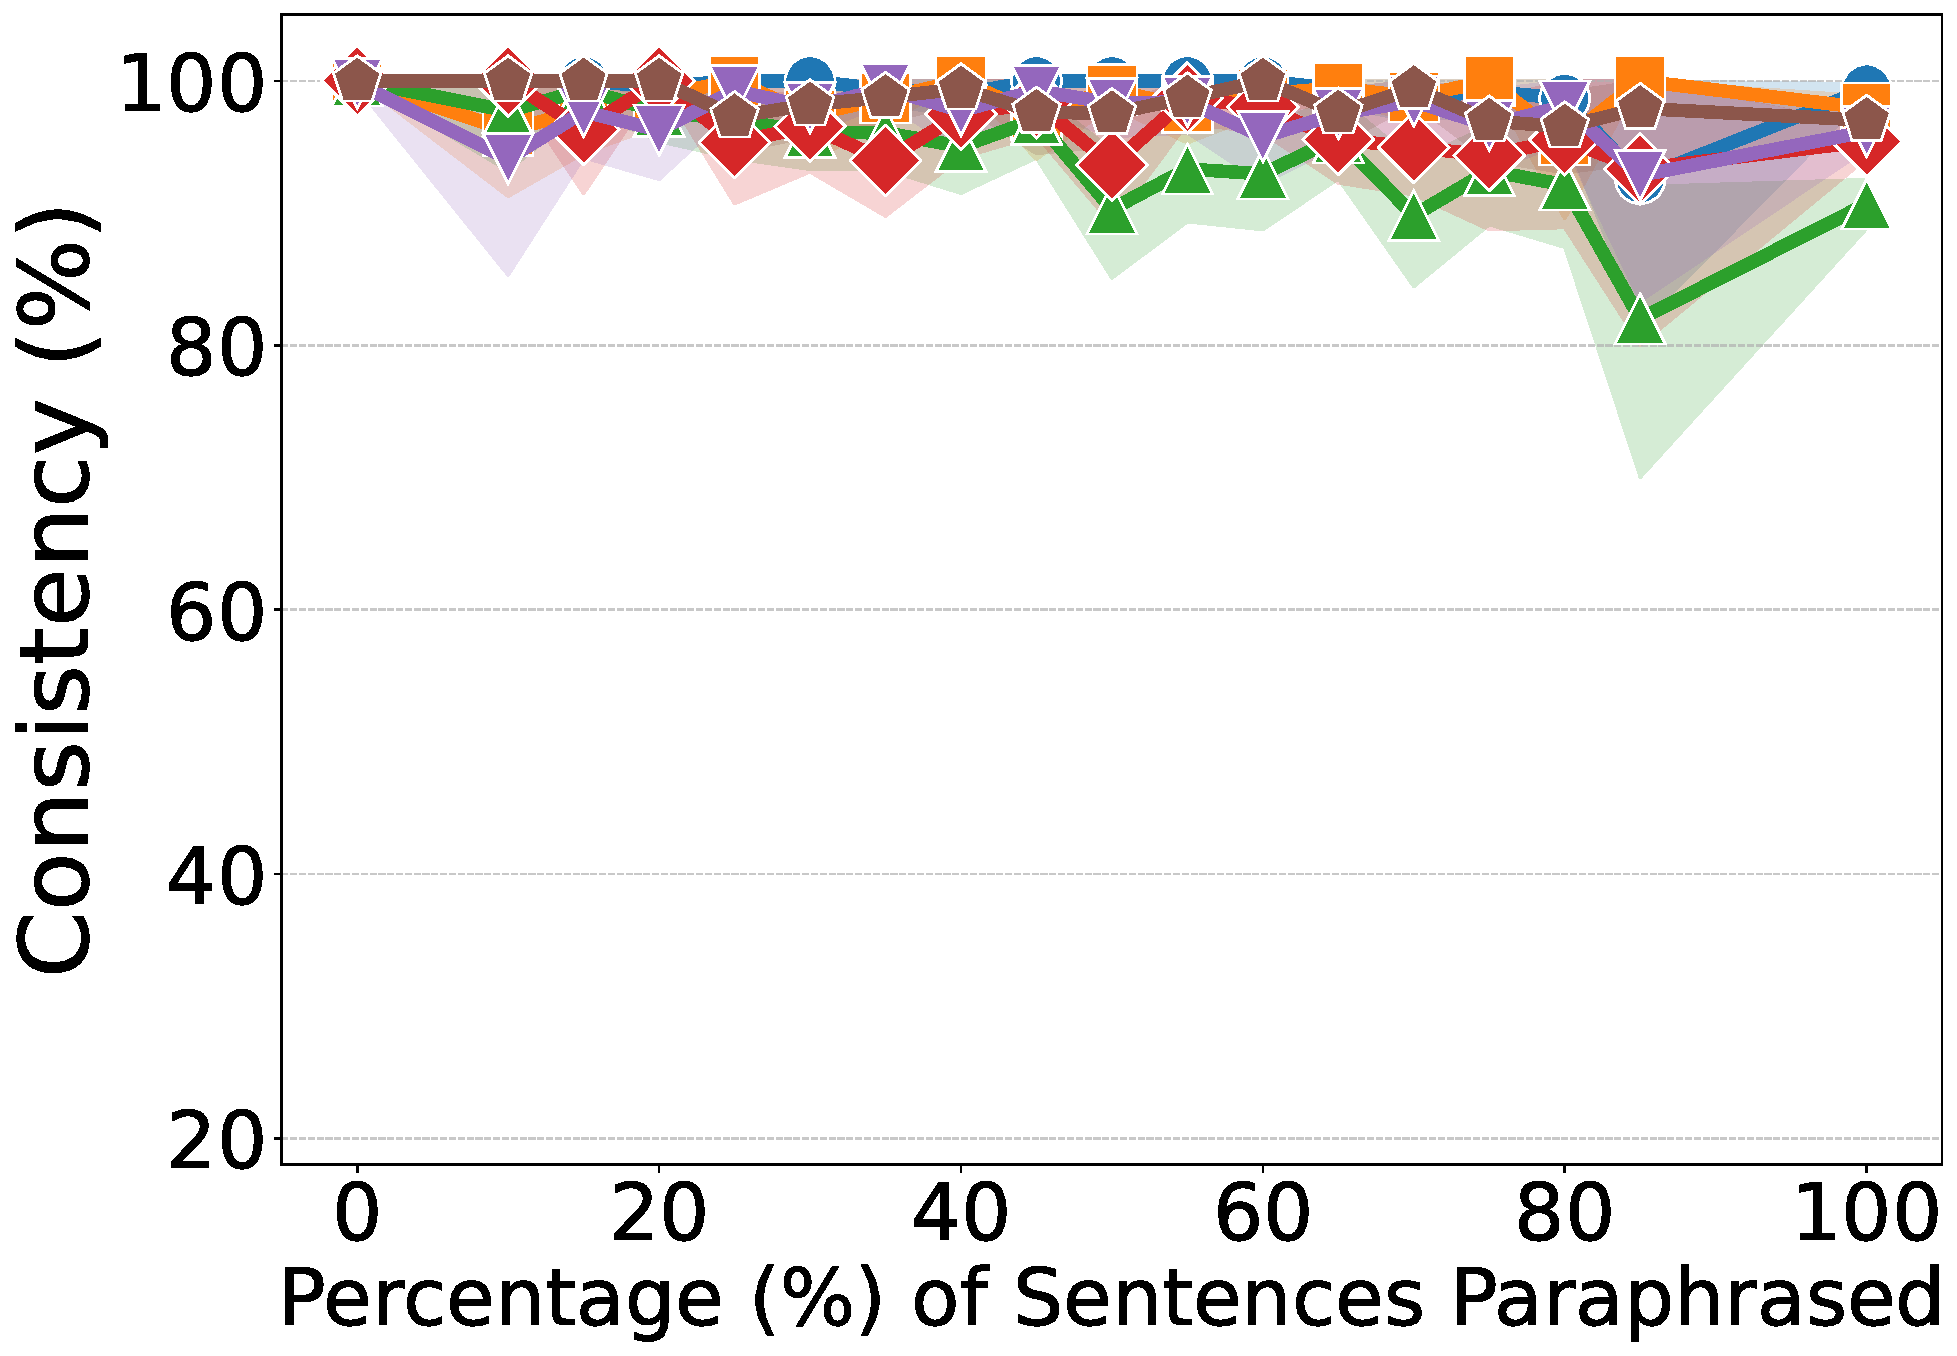
\includegraphics[width=\figsize\textwidth]{figures/cot_intervention/qwen_omni/paraphrasing/cross_dataset_paraphrasing_0pct_words_qwen_omni_restricted-mistral.pdf} %\hfill
    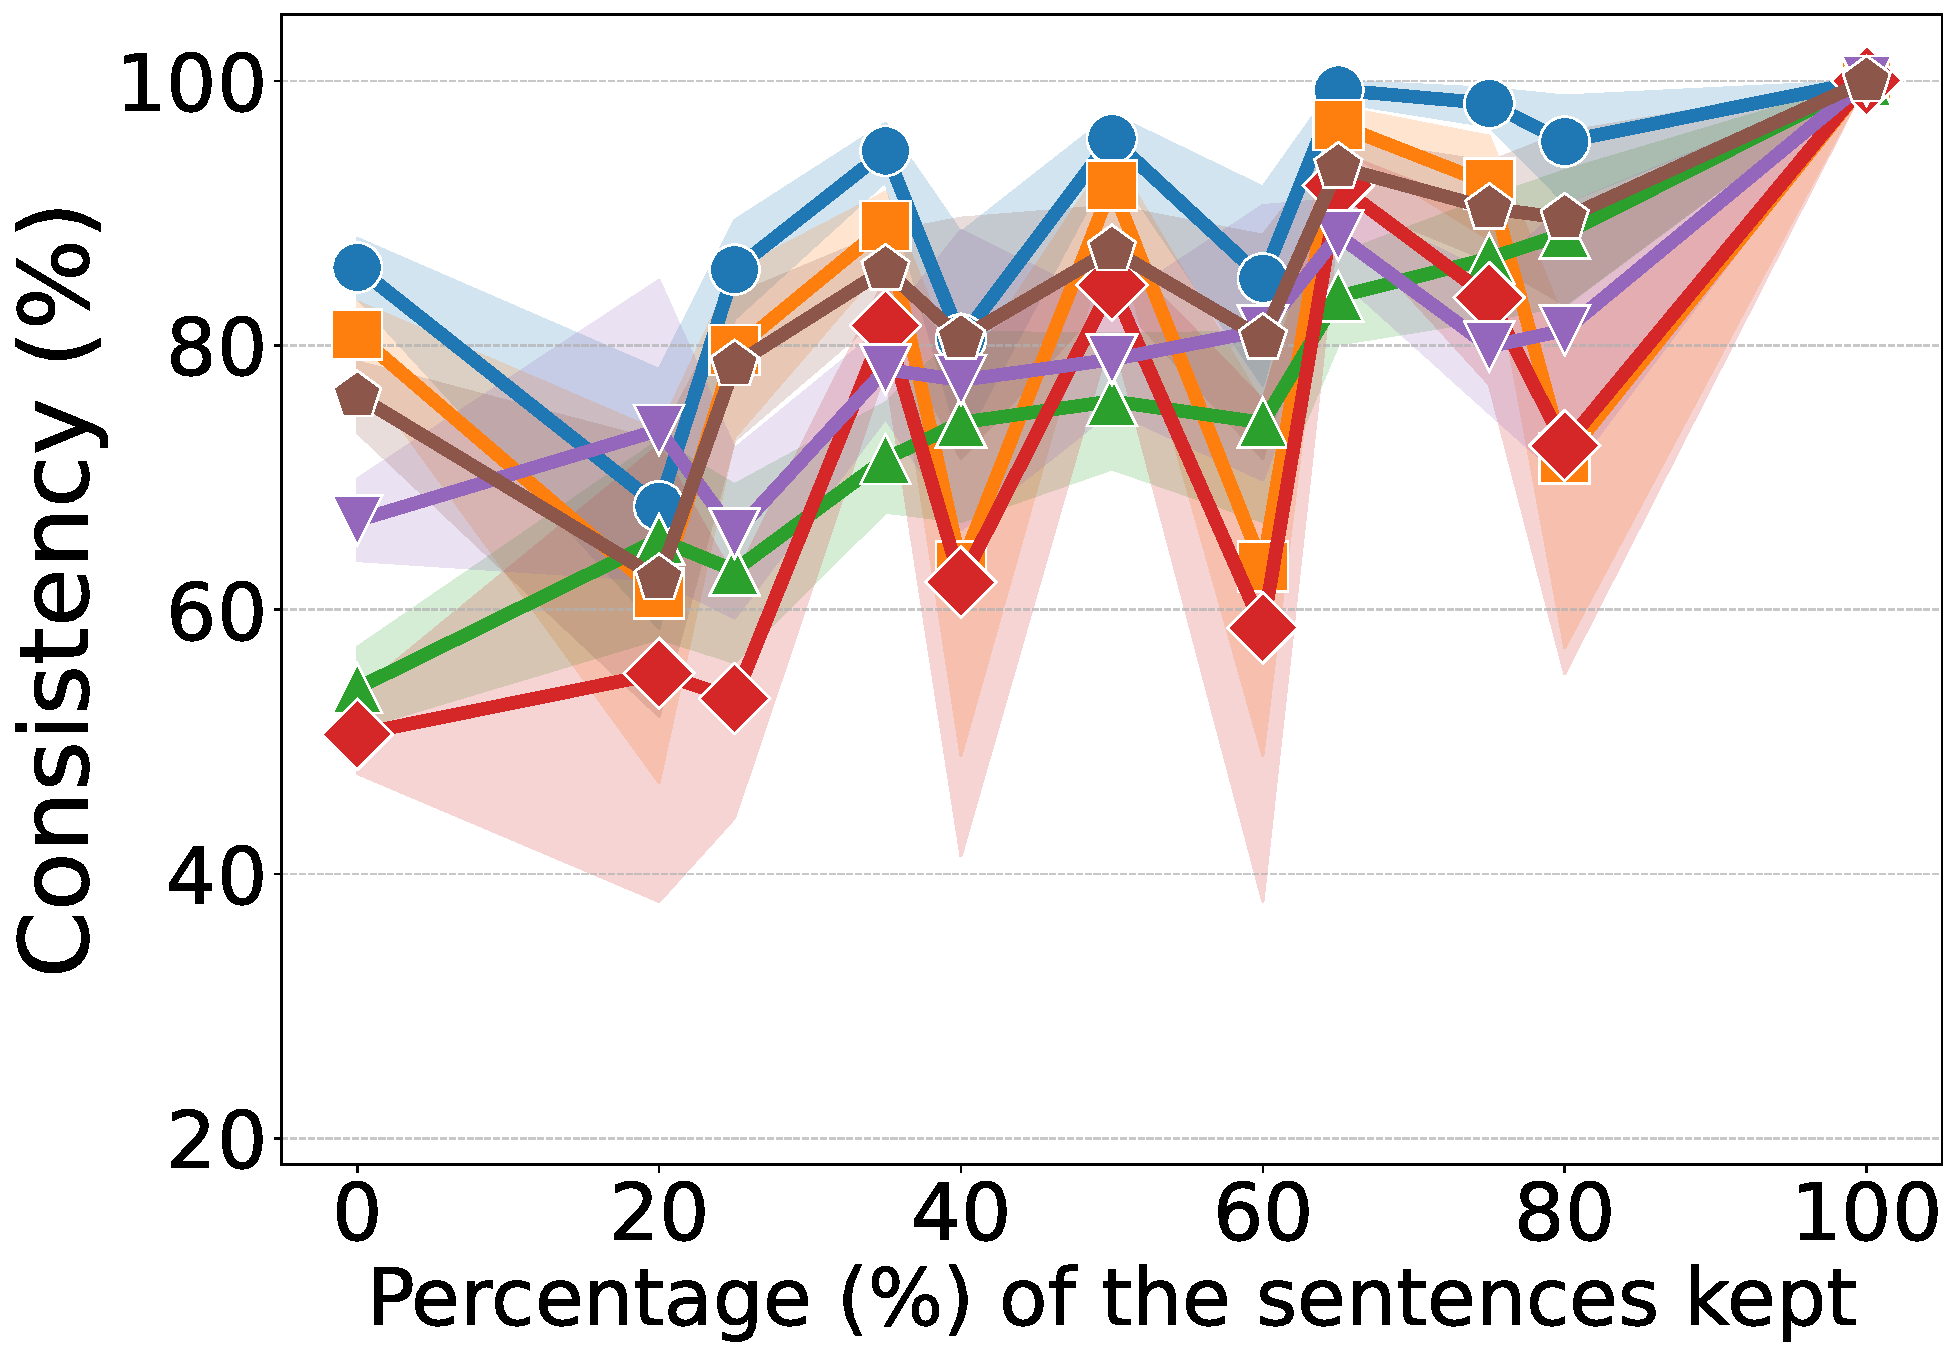
\includegraphics[width=\figsize\textwidth]{figures/cot_intervention/qwen_omni/early_answering/cross_dataset_early_answering_100pct_qwen_omni_restricted.pdf} %\hfill
    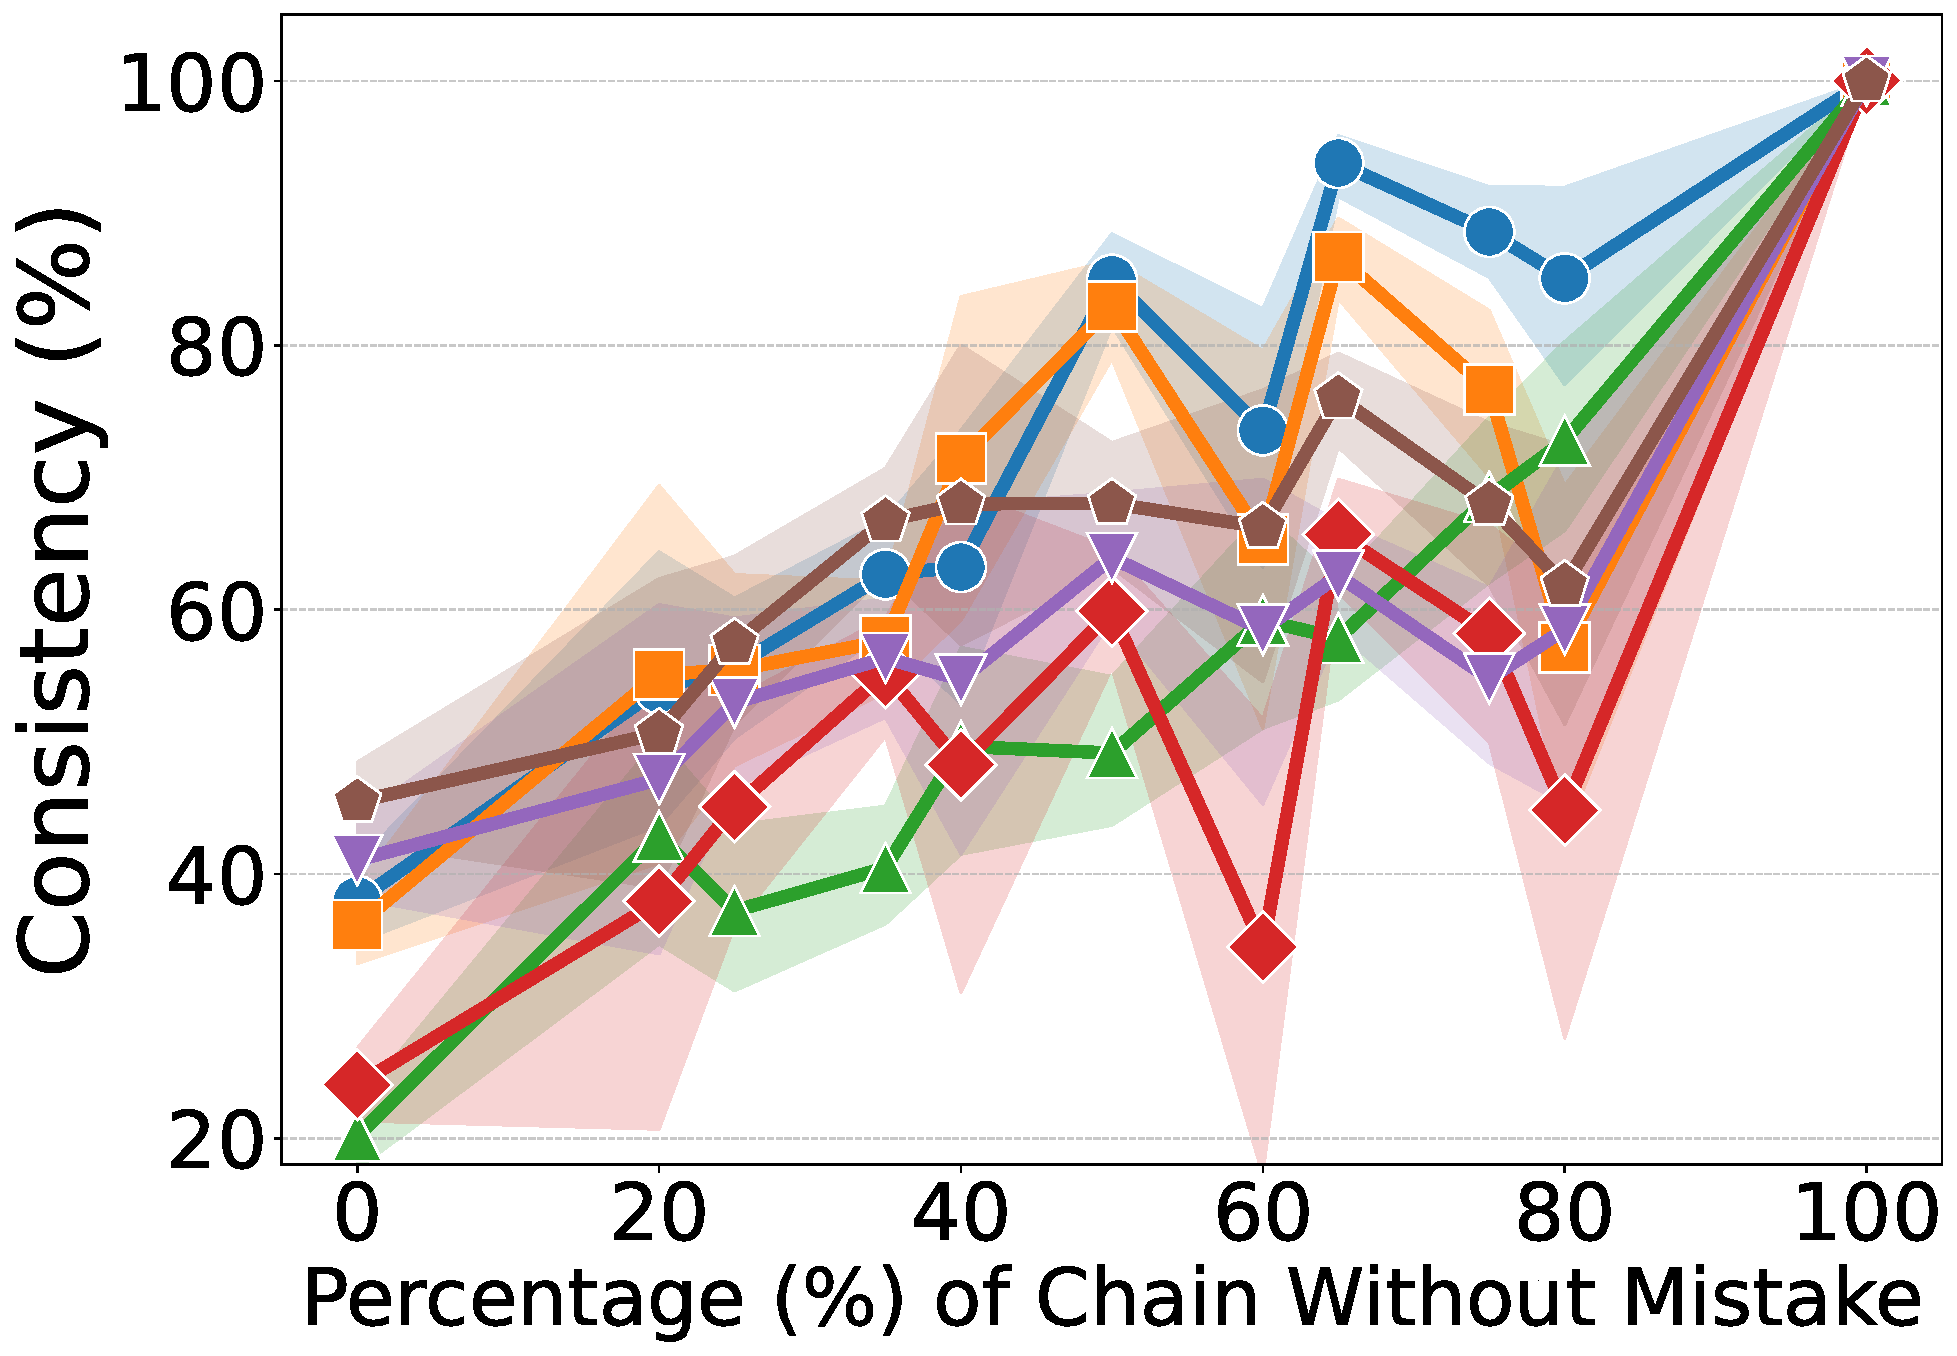
\includegraphics[width=\figsize\textwidth]{figures/cot_intervention/qwen_omni/adding_mistakes/cross_dataset_adding_mistakes_vs_rpf_qwen_omni_restricted-mistral.pdf}% \hfill
    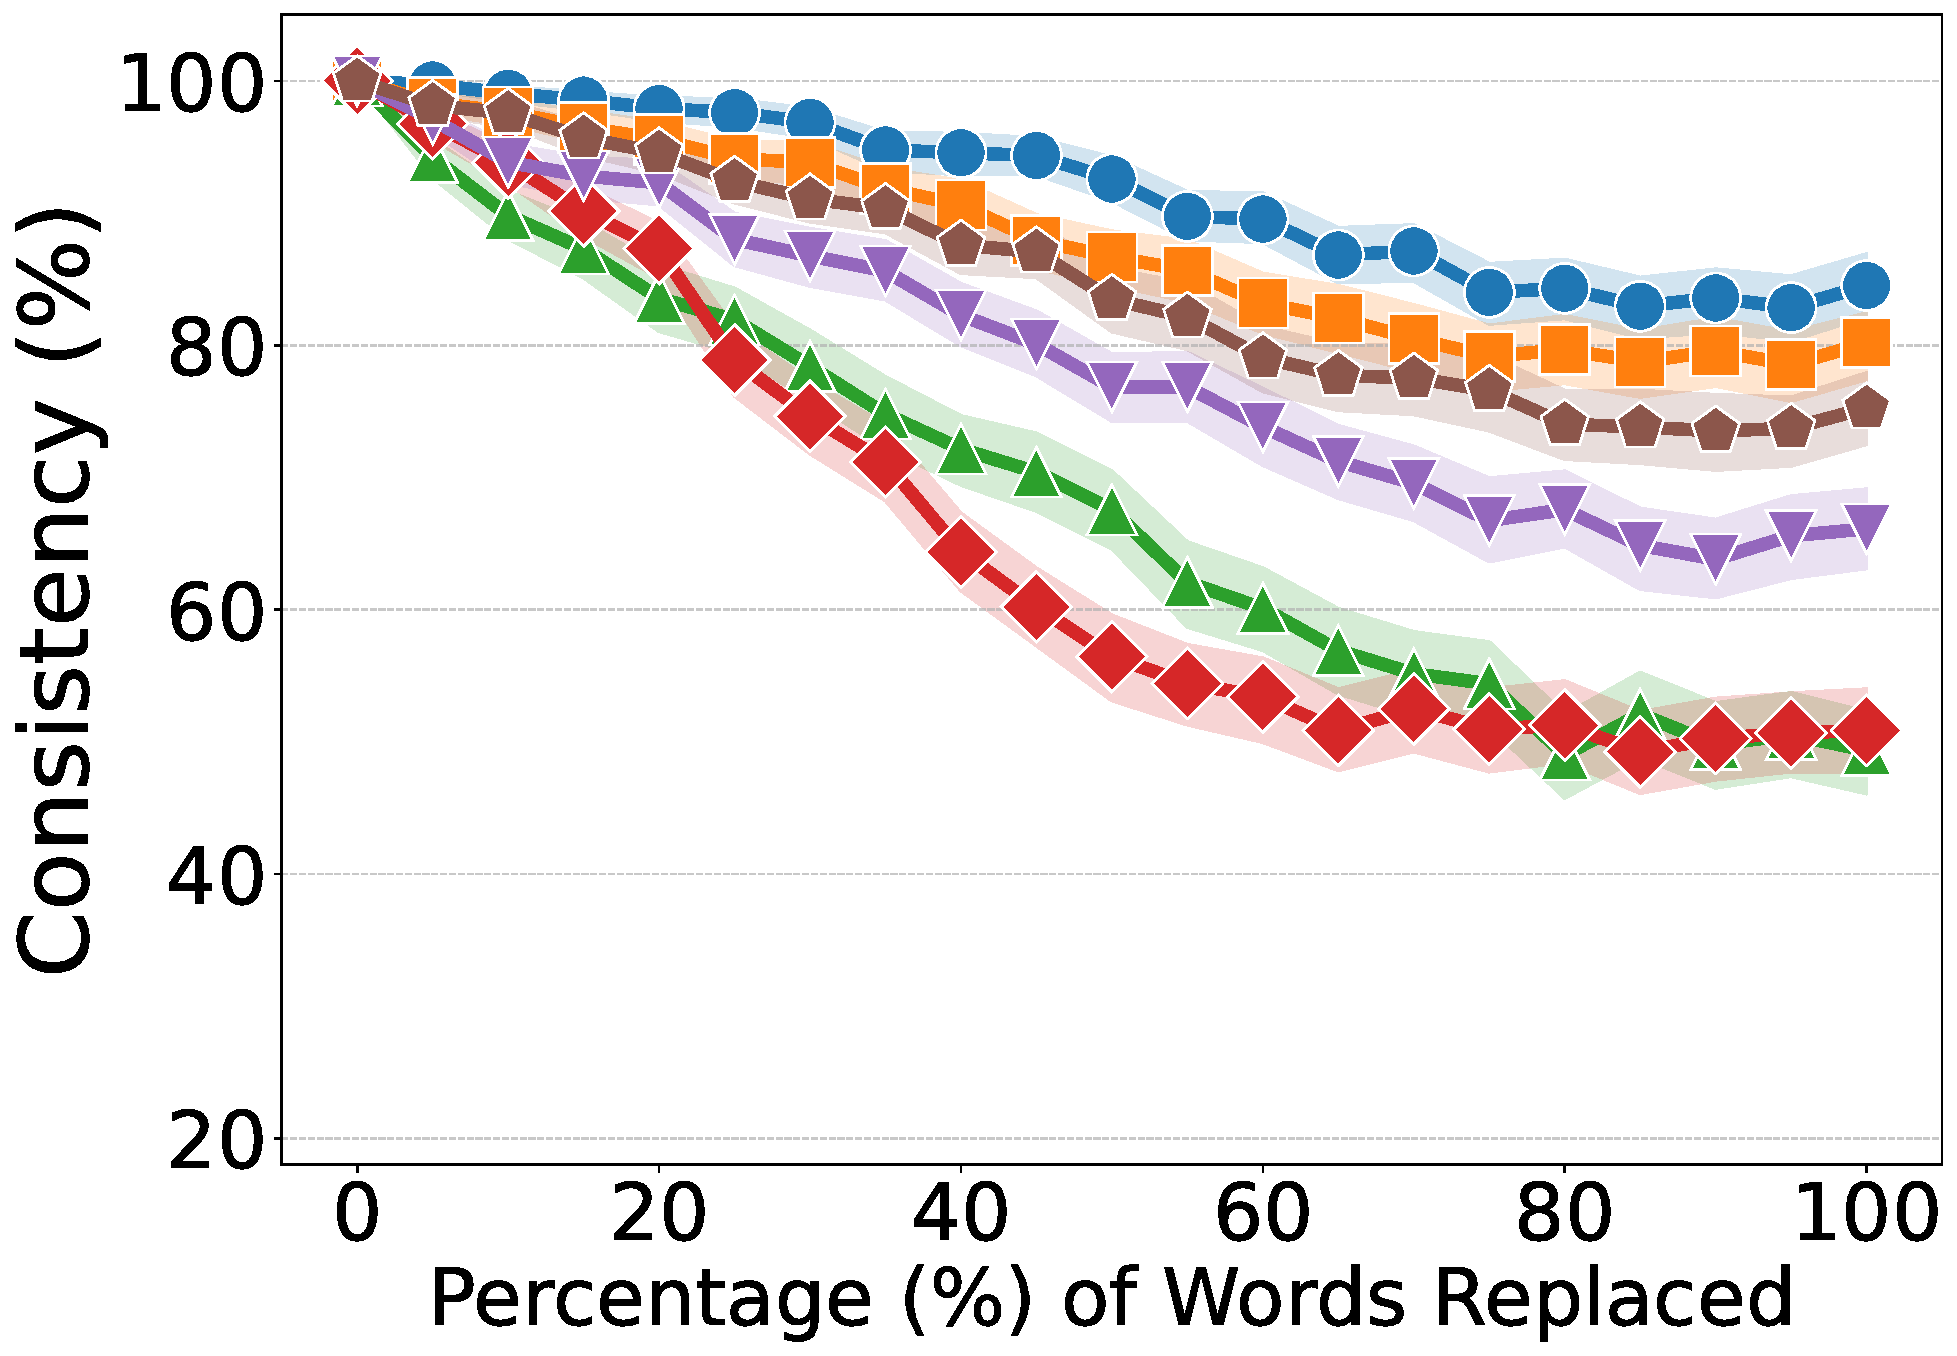
\includegraphics[width=\figsize\textwidth]{figures/cot_intervention/qwen_omni/random_partial_filler_text/cross_dataset_random_partial_filler_text_0pct_qwen_omni_lorem_restricted.pdf}
    
    \caption{CoT Interventions. \textbf{(left)} Paraphrasing, \textbf{(mid-left)} Early Answering, \textbf{(mid-right)} Adding Mistakes, \textbf{(right)} Filler Tokens} 
    \vspace{-.4cm}
    \label{fig:cot_intervention_grid}
\end{figure*}


\noindent \textbf{Results:} 
The accuracy and consistency plots in Figure \ref{fig:full_results_quantitative audio} show that both models remain stable up to a 60\% random masking ratio but fail significantly at higher ratios. Figure \ref{fig:jasco_result} further reveals a clear imbalance in how the models process multimodal inputs: guided masking shows that they do not listen wholistically (Q2) and instead rely heavily on speech. The mean similarity scores and modality bars suggest that the models attempt to adjust their reasoning depending on which modality remains available—referring more to audio when speech is masked and vice versa, but performance still drops under any guided intervention. Interestingly, masking general audio while keeping speech leads to lower similarity scores. This likely occurs because the model can more easily hallucinate details from spoken context than infer information from background sounds. Table \ref{tab:cot_consistency} further shows that AF3 often produces hallucinatory reasoning when the input is silent. At 100\% masking, it still maintains a consistency score of 3.65 on MMAU. In contrast, Qwen2.5-Omni remains more grounded and frequently reports that it cannot hear an audible signal. This behavior leads to lower consistency scores (e.g., 2.35 on SAKURA-Animal) but reduces hallucinated reasoning.

    %\caption{\textbf{Modality Dependency under Guided Masking.} The values in parentheses on the left indicate the mean similarity score compared to the reference answers. The percentages above the bars represent the proportion of responses that are audio-dependent (A), both-dependent (A-S), and speech-dependent (S).}
    %\label{fig:jasco_result}
%\end{figure}

% Regarding \textbf{Q1}, Table \ref{tab:cot_consistency} indicates that AF3 frequently hallucinates reasoning for silent inputs. At 100\% masking, AF3 produces a CoT that appears "consistent" with a real answer, scoring 3.65 on MMAU. In contrast, Qwen2.5-Omni is more grounded; its CoT often correctly states it cannot hear an audible signal, leading to lower consistency scores (e.g., 2.35 on SAKURA-Animal).

% Your results text or table goes here.
\begin{figure}[htb]
    \centering
    % Left Figure: AF3
    \begin{subfigure}{0.48\columnwidth}
        \centering
        \textbf{Audio Flamingo 3 (AF3)}\\[0.2em]
        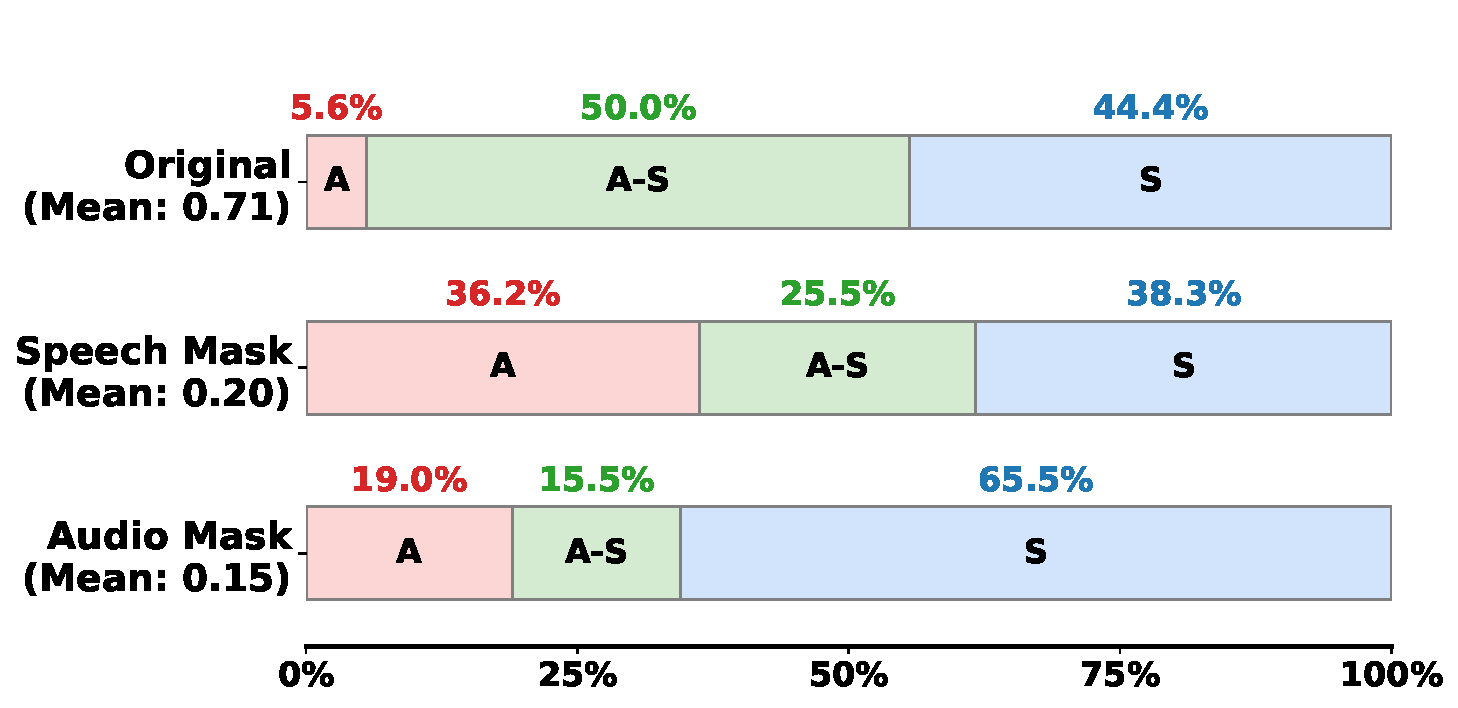
\includegraphics[width=\linewidth]{figures/audio_intervention/af3_modality_dependence.pdf}
        \label{fig:af3_bar_scaled}
    \end{subfigure}
    \hfill % This horizontal fill puts them side-by-side
    % Right Figure: Qwen2.5-Omni
    \begin{subfigure}{0.48\columnwidth}
        \centering
        \textbf{Qwen2.5-Omni}\\[0.2em]
        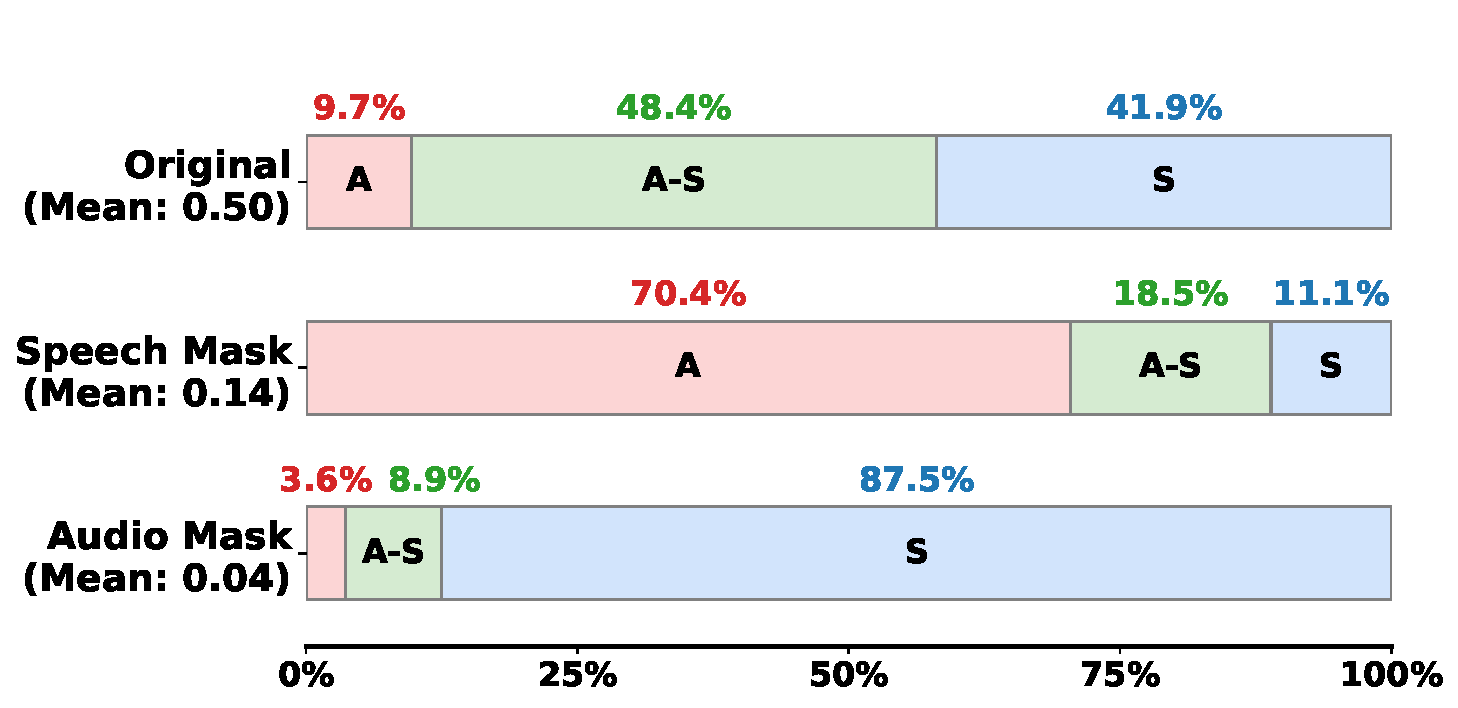
\includegraphics[width=\linewidth]{figures/audio_intervention/qwen_modality_dependence.pdf}
        \label{fig:qwen_bar_scaled}
    \end{subfigure}
    \vspace{-.4cm}
    \caption{\textbf{Modality Dependency under Guided Masking.} The values in parentheses (on the left) indicate the mean similarity score compared to the reference answers. The percentages above the bars represent the proportion of responses that are audio-dependent (A), both-dependent (A-S), and speech-dependent (S).}
    \vspace{-.6cm}
    \label{fig:jasco_result}
\end{figure}

%\noindent \textbf{Results:} 
%The accuracy and consistency plots in Figure \ref{fig:full_results_quantitative audio} show that while models are stable up to 60\% random masking, they exhibit failures at higher ratios. As shown in Figure \ref{fig:jasco_result}, masking different parts of the audio reveals a clear imbalance in how models listen. For Q2, both models rely much more on speech than on general audio. When we mask only the general audio (keeping speech), Qwen2.5 still yields 87.5\% correct reasoning based solely on speech, while AF3 relies on speech for 65.5\% of its correct outputs. When speech is masked, performance drops significantly for both models (Mean 0.20 for AF3 and 0.14 for Qwen), proving they do not listen "wholistically" and are heavily biased toward speech.
%
%Regarding Q1, Table \ref{tab:cot_consistency} shows that AF3 often hallucinates reasoning for silent inputs. At 100\% masking (total silence), AF3 still produces a CoT that appears "consistent" with a real answer, scoring 3.65 on MMAU. In contrast, Qwen2.5 is more honest; its CoT often states it cannot hear anything, leading to lower consistency scores (e.g., 2.35 on SAKURA-Animal) but fewer hallucinations.

